\documentclass[utf8x]{ctexart}
\usepackage{setspace}
\usepackage{url}
\onehalfspacing
\usepackage{amsmath,amssymb,amsfonts,amsthm,mathtools}
\usepackage[english]{babel}
\usepackage[T1]{fontenc}
\usepackage{lmodern}
\usepackage{dsfont}
\usepackage{bbm}
\usepackage[round]{natbib}
\usepackage{color} 
\usepackage[defaultlines=2,all]{nowidow}
\usepackage{caption}
\usepackage[labelformat=simple]{subcaption}
\usepackage{makecell}
\renewcommand\thesubfigure{(\alph{subfigure})}

\setlength\parindent{0pt}
\setlength{\parskip}{6pt plus 1pt minus 1pt}

\newcommand{\red}{\textcolor{red}}


\begin{document}

\begin{titlepage}
    \centering
    {\scshape\LARGE National Taiwan University \par}
    \vspace{1cm}
    {\scshape\Large Financial Technology \par}
    \vspace{2cm}
    {\huge\bfseries Project 2: Stock Price Prediction \par}
    \vspace{2cm}
    {\Large Lecturer:\\
        Che Lin (林澤) \par}
    \vspace{1cm}
    {\Large Author: Tadeo Hepperle, Student ID: A11922105 \par}
    \vfill
    {\large \today\par}
\end{titlepage}


\tableofcontents

\cleardoublepage

\section{Introduction}

In this project historical data on the Apple Inc. stock is used to predict the stocks price on the next day. This is a regression task for which we are going to compare multiple methods:
\begin{itemize}
    \item A simple model always using the current days Close price to predict the next day's Close price.
    \item A moving average model, that predicts the next day's Close price by a learned linear combination of the past 30 Close prices.
    \item A Recurrent Neural Network with one layer
    \item An LSTM model
    \item A GRU model
\end{itemize}

\subsection{Description of the data}

The dataset contains various technical features concerning the Apple Inc. stock price in the time interval between 2011/01/03 and 201/12/31 a total of 754 data points.
For each data point the following 6 features are available:
\begin{itemize}
    \item Open - price of the stock when markets opened
    \item High - highest price of the stock on that day
    \item Low - lowest price of the stock on that day
    \item Close - price of the stock when markets closed
    \item Volume - the total volume of the stock traded
    \item Adjusted Close - stock's value after accounting for any corporate actions
\end{itemize}

In addition to these inherent features, 5 other features were computed:
\begin{itemize}
    \item MA10 - 10 day moving average
    \item MA30 - 30 day moving average
    \item K - from the KD-indicator line chart
    \item D - from the KD-indicator line chart
    \item Weekday - one hot encoded into 7 different binary features
\end{itemize}

The data points are continous without gaps except for weekends and other days where the stock market is closed.
For method selection and model evaluation the data was split into train, validation and test sets:
\begin{itemize}
    \item Train set - stock price from 2011/01/01 - 2012/12/31
    \item Validation set - stock price from 2013/01/01 - 2013/06/30
    \item Test set - stock price from 2013/07/01 - 2013/12/30
\end{itemize}


\subsection{Description of methods}







\subsubsection{Last Value Model}

The simplest model to predict the next day's Close price is to just use the current day's Close price as the prediction. This model does not need any training and can be understood as a baseline model other models can be compared to in terms of their train and test loss.

\subsubsection{Moving Average Model}

A moving average in it's more general definition is a linear combination of the values a subsequence of the sequence. In this model we want to form a linear combination of the past 30 Close values to predict the next Close price. For this we need to learn 30 weights.

\subsubsection{Recurrent Neural Network}

The recurrent neural network (RNN) is specified by 2 parameters: $input_size$ and $hidden_size$. In this project we always just use an RNN with 1 layer. The RNN learns over a period of $time_steps = 30$ iterations. In each iteration, an input vector of size $input_size$ and a hidden state vector of size $hidden_size$ are concatinated into a combined vector which is fed through a ReLU-activated linear layer to produce the hidden state for the next iteration. In the initial iteration the hidden state is a zero-vector. After the $time_steps$ iterations of this process, the hidden state is mapped by a linear layer to a single scalar value (the Close price we want to predict).
Mini-batch gradient descent is used to train such an RNN.

\subsubsection{LSTM}

LSTM stands for long short-term memory. The LSTM tries to improve on the RNN by using a cell state in addition to the hidden state, which is also a vector of $hidden_size$. while the hidden state represents a short term memory because the gradients deteriorate over time, the cell state is connected via constant gradient flow and can store information for much longer.

\begin{math}
    \begin{aligned}f_{t}            & =\sigma _{g}(W_{f}x_{t}+U_{f}h_{t-1}+b_{f})     \\
               i_{t}            & =\sigma _{g}(W_{i}x_{t}+U_{i}h_{t-1}+b_{i})     \\
               o_{t}            & =\sigma _{g}(W_{o}x_{t}+U_{o}h_{t-1}+b_{o})     \\
               {\tilde {c}}_{t} & =\sigma _{c}(W_{c}x_{t}+U_{c}h_{t-1}+b_{c})     \\
               c_{t}            & =f_{t}\odot c_{t-1}+i_{t}\odot {\tilde {c}}_{t} \\
               h_{t}            & =o_{t}\odot \sigma _{h}(c_{t})
    \end{aligned}
\end{math}

in the equation abobe $x_t$ stands for the input feature vector at a given time $t$ starting from $t = 1$ up to $t = 30$ in our case. $h_t$ represents the hidden state, while $c_t$ is the cell state. In each iteration of the forward pass the formulas above are applied, to generate a new $h_t$ and $c_t$ until finally $h_{30}$ is mapped my a linear layer to a single scalar: the predicted Close value of the next day.

In theory, one could have multiple layers in each iteration, we will just use 1-layer LSTMs and GRUs in this project.

\subsubsection{GRU}

GRU stands for gated recurrent unit. In comparison to the LSTM it lacks the input/update gate and the cell state but has been found to produce similar results at a lower computational cost in many applications. In each forward pass the following formulas are applied to get from the input $x_t$ and the hidden state $h_t$ to the next hidden state:


\begin{math}
    \begin{aligned}z_{t}          & =\sigma _{g}(W_{z}x_{t}+U_{z}h_{t-1}+b_{z})            \\
               r_{t}          & =\sigma _{g}(W_{r}x_{t}+U_{r}h_{t-1}+b_{r})            \\
               {\hat {h}}_{t} & =\phi _{h}(W_{h}x_{t}+U_{h}(r_{t}\odot h_{t-1})+b_{h}) \\
               h_{t}          & =z_{t}\odot {\hat {h}}_{t}+(1-z_{t})\odot h_{t-1}\end{aligned}
\end{math}

\section{Results}

First we will provide descriptive statistics and graphics of the dataset before moving on to compare the regression methods with each other.

\subsection{Descriptive Statistics}

The price of the Apple Inc. stock fluctuated between \$67.9 and \$134.1 in the given time frame. A volume between \$800.000 and \$15.000.000 was traded every active day.
The 3 charts in Figure~\ref{fig:candles} display the price development, traded volume and KD-line in the entire timeframe of almost 2 years.

In the topmost candle-chart the blue line represents the 10-Day moving average, while the orange line is the 30-Day moving average.

In the bottom chart shows the K (blue line) and D statistics (orange line), both common technical indicators.

\label{fig:candles}
\begin{figure}[p]
    \vspace*{-2cm}
    \makebox[\linewidth]{
        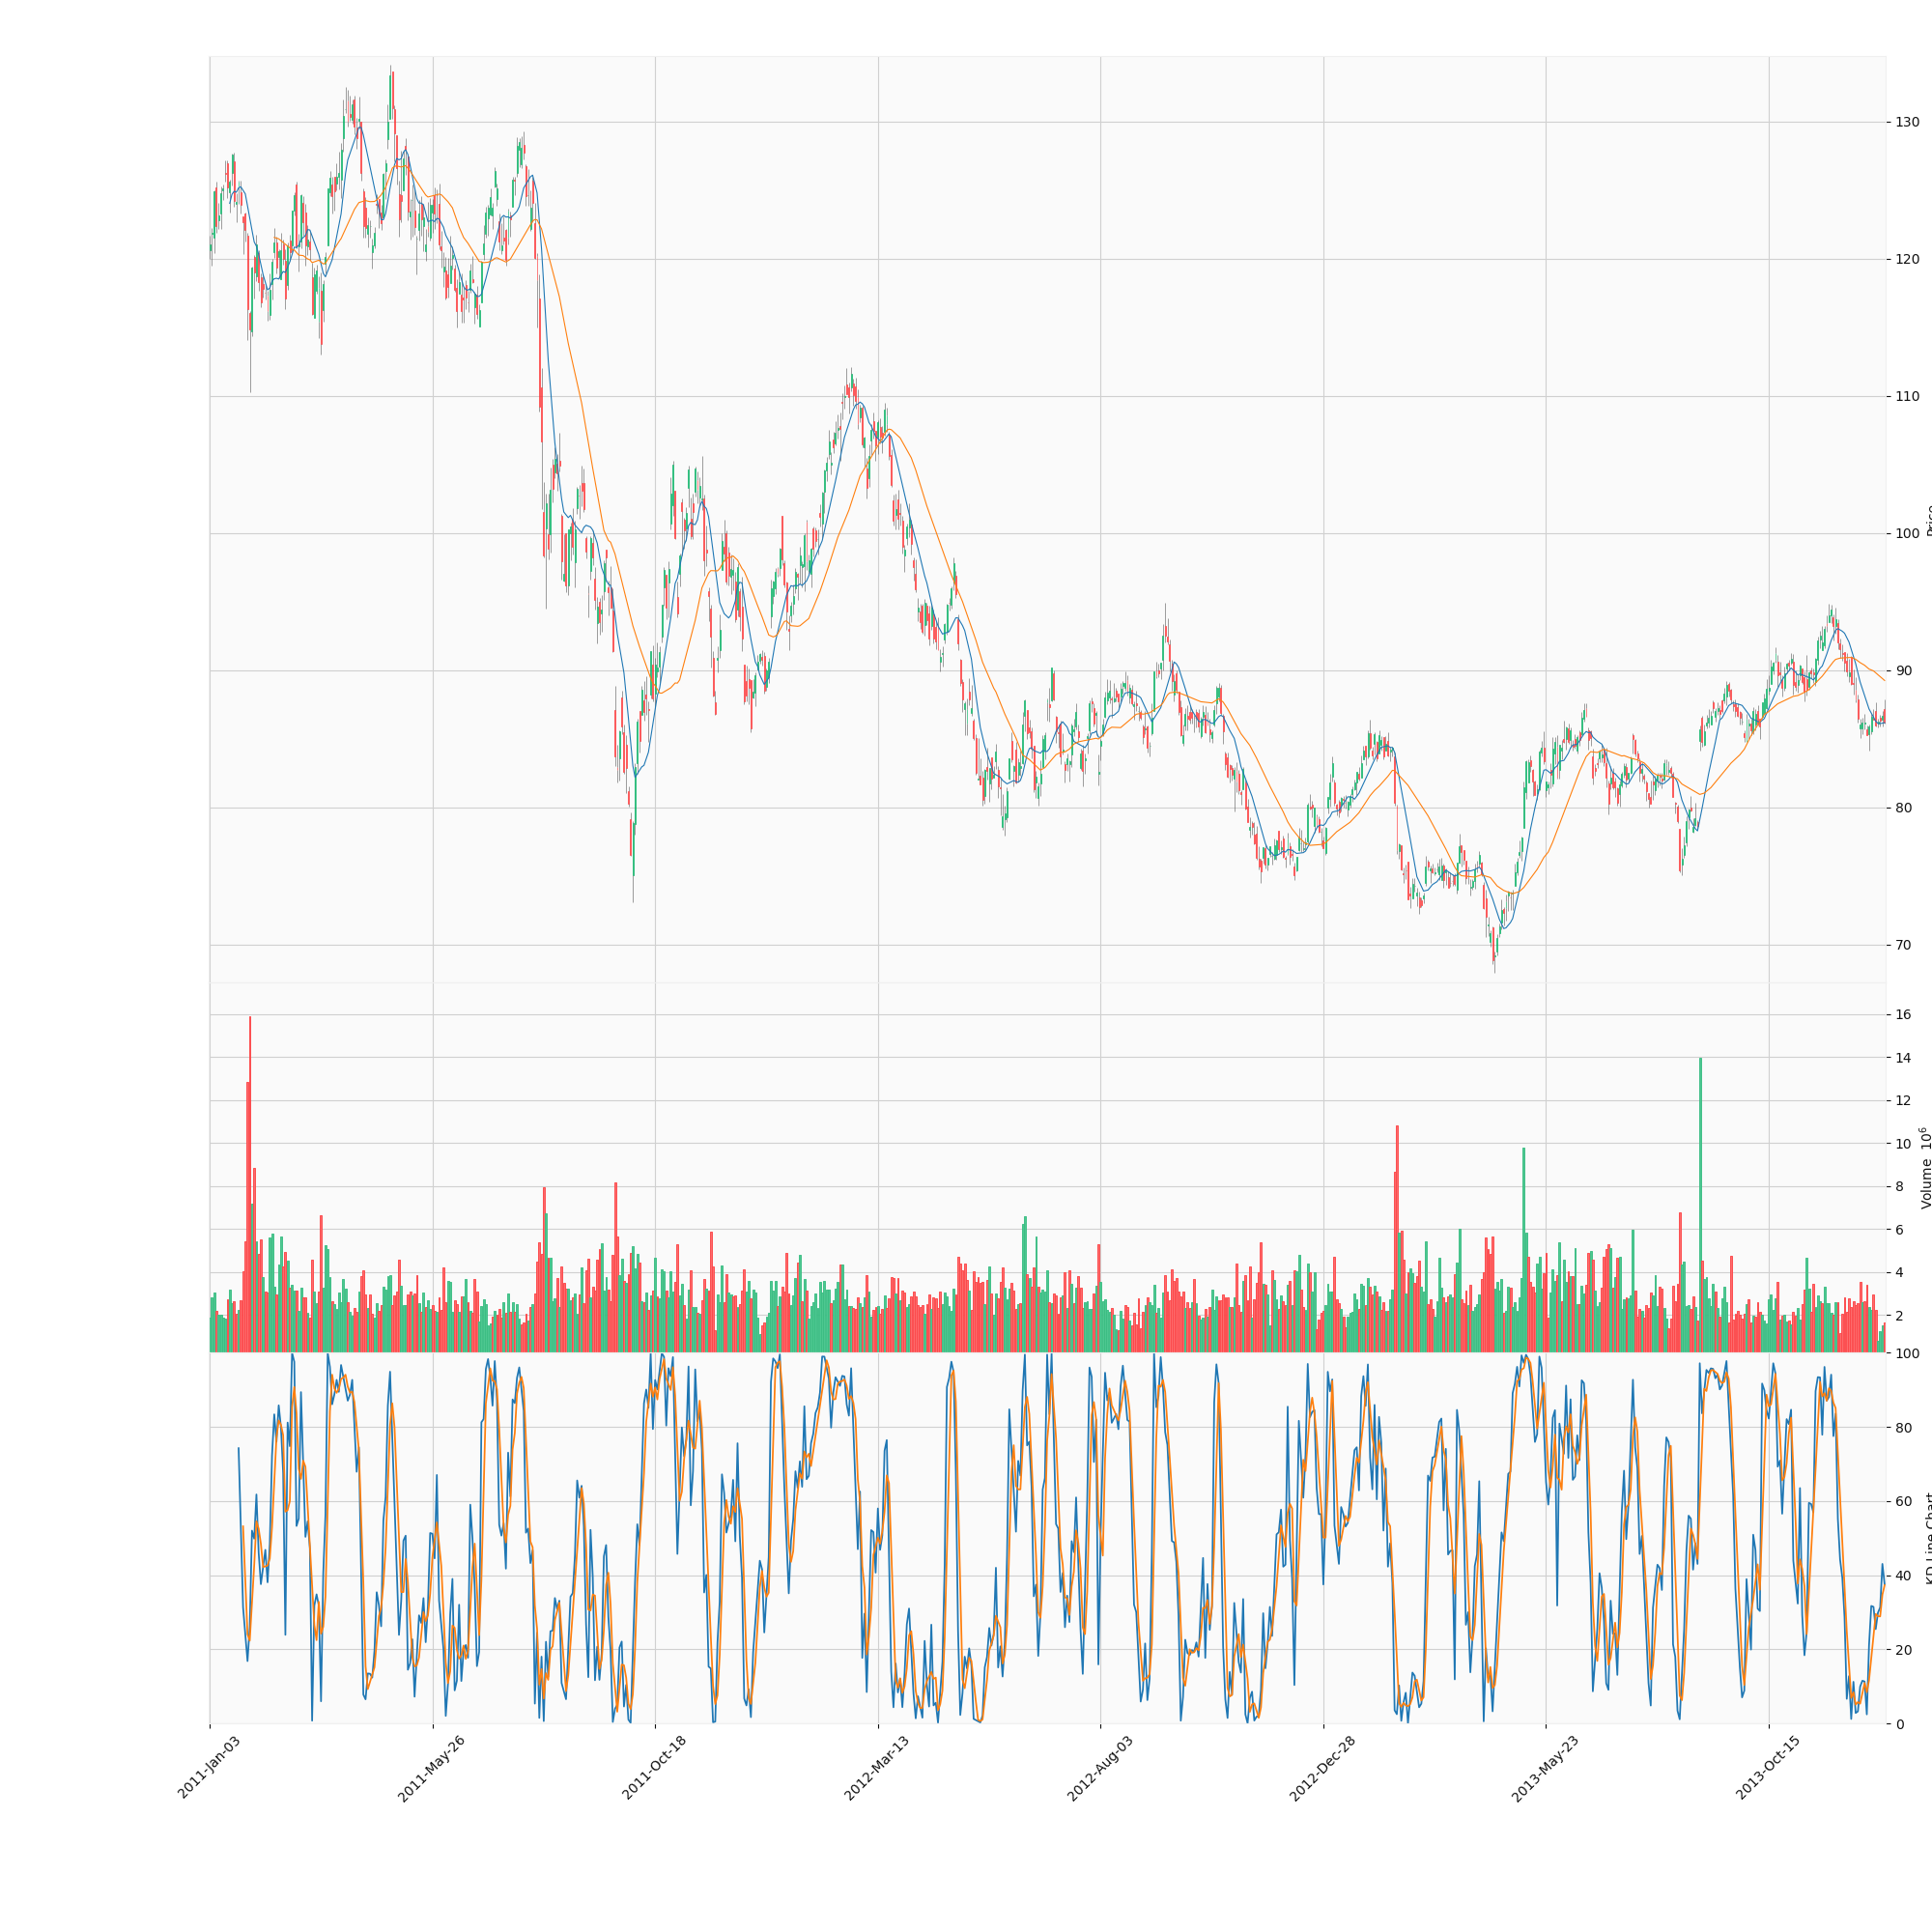
\includegraphics[width=1.3\linewidth]{../images/candles_KD_volume.png}
    }
    \caption{Sequence diagram}
\end{figure}

Before applying any prediction model the features and labels (Close price of the next day) were min-max normalized to a range between 0 and 1. The weekdays were computed from the date and one-hot-encoded.

\subsection{Last Value Model}

As a baseline for all further learning we need to know how well we can predict the next Close price with a very simple model: What if we just take the last day's Close price as the prediction?
Such a model yields results on the 3 data set slices like displayed in Table~\ref{tab:last_value_model} and gives price predictions like shown in Figure~\ref{fig:last_value_model}.

\begin{figure}[htb]
    \centering
    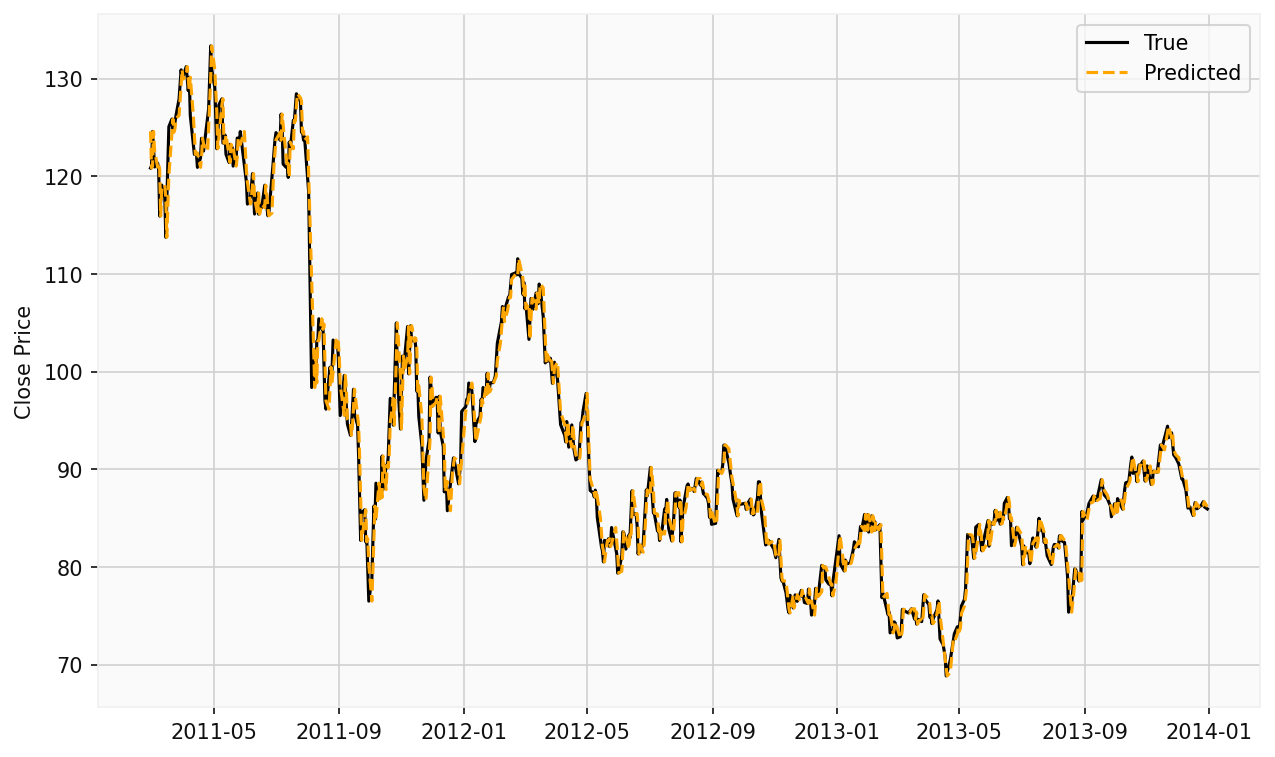
\includegraphics[width=\textwidth]{../images/last_value_model.png}
    \caption{Predictions of the Last Value Model}
    \label{fig:last_value_model}
\end{figure}

\begin{table}[ht]
    \centering
    \caption{MSE of the Last Value Model on train, valaidation and test set}
    \label{tab:last_value_model}
    \begin{tabular}{c|ccc}
            & Train set & Validation set & Test set \\
        \hline
        MSE & 0.00102   & 0.00035        & 0.00028  \\
    \end{tabular}
\end{table}

It will be compared to other models below.

\subsection{Moving Average Model}

Pytorch was used to train a neural network with 1 linaer layer that models the next Close Price as a Moving Average of the last 30 days with variable weights. The weights were initialized to resemble the Last Value model at first, s.t. $w = [0,0,0,\dots,1]$ and $Card(w) = 30$.




\section{Discussion}

\end{document}
